\documentclass[12pt, oneside]{article} 
\usepackage{amsmath, amsthm, amssymb, calrsfs, wasysym, verbatim, bbm, color, graphics, geometry, multirow, booktabs}
\usepackage{graphicx}
\usepackage{tikz}
\usepackage{amsmath}
\usepackage{graphicx}
\usepackage{amsmath, amssymb, amsthm}
\usepackage{setspace}
\usepackage{tikz}
\usetikzlibrary{trees, positioning}
\usepackage{pgfplots}
\renewcommand{\baselinestretch}{1.0}
\geometry{tmargin=.75in, bmargin=.75in, lmargin=.75in, rmargin = .75in}  

\newcommand{\R}{\mathbb{R}}
\newcommand{\C}{\mathbb{C}}
\newcommand{\Z}{\mathbb{Z}}
\newcommand{\N}{\mathbb{N}}
\newcommand{\Q}{\mathbb{Q}}
\newcommand{\Cdot}{\boldsymbol{\cdot}}


\title{SP25 7130: Homework 2}
\author{Danbo CHEN}
\date{\today}

\begin{document}

\maketitle
\vspace{.25in}

\section{Question 1.4}
\textbf{(4) Solution:}
\subsection{Summary of Findings}
\textbf{1. Program Impact on Expenditures}  
\begin{itemize}
    \item \textbf{Non-food expenditures increased significantly} ($\beta_1 = 28.844$, $p < 0.05$).
    \item \textbf{No significant effect on food expenditures} after adding baseline controls.
\end{itemize}

\textbf{2. Role of Baseline Covariates}  
\begin{itemize}
    \item \textbf{Household size} increases both \textbf{food} (+50.73, $p < 0.01$) and \textbf{non-food} (+14.19, $p < 0.01$) expenditures.
    \item \textbf{Education increases non-food spending} ($\beta_3 = 11.624$, $p < 0.01$).
    \item \textbf{Remittances increase non-food expenditures} ($\beta_5 = 0.896$, $p < 0.01$), but have no effect on food expenditures.
\end{itemize}

\textbf{3. Econometric Concerns}  
\begin{itemize}
    \item \textbf{Omitted variable bias (OVB)}: The simple ITT model \textbf{overestimated} the treatment effect on food expenditures.
    \item \textbf{Low $R^2$ values}: Even after adding controls, \textbf{unobserved factors drive expenditures}.
    \item \textbf{Potential endogeneity}: Treatment assignment may correlate with \textbf{unobserved household characteristics}.
\end{itemize}

\textbf{4. Policy Implications}  
\begin{itemize}
    \item \textbf{Cash transfers increase non-food spending}, supporting broader welfare needs.
    \item \textbf{Larger households spend more}; transfers should \textbf{consider household size}.
    \item \textbf{Education and remittances shape financial decisions}, suggesting \textbf{long-term benefits} from cash transfers.
\end{itemize}

\textbf{Conclusion}
The cash transfer program effectively increased \textbf{non-food expenditures}, but its impact on \textbf{food expenditures is limited}. Future studies should explore \textbf{heterogeneous effects} and potential \textbf{long-term benefits}.

\section{Question 3.1}
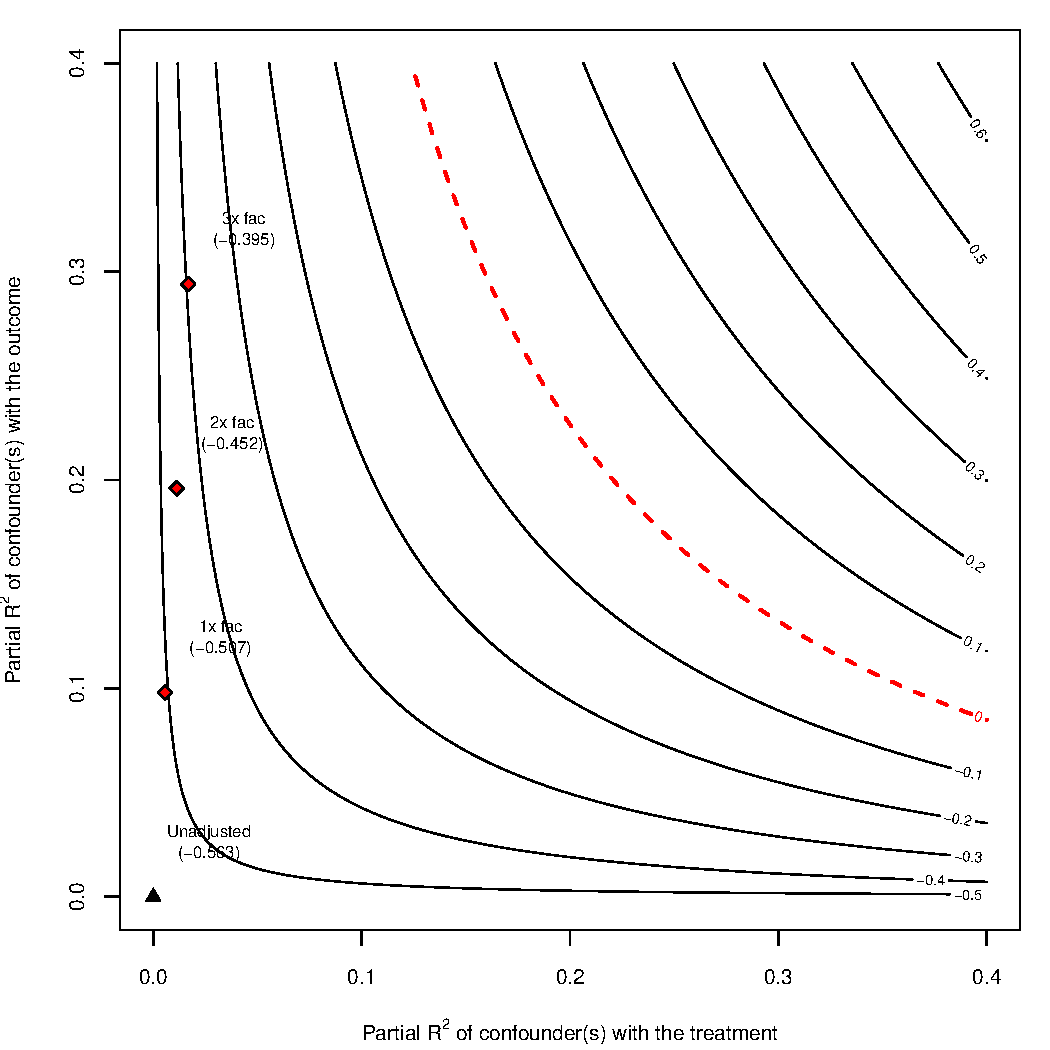
\includegraphics[]{Rplots.pdf}
\begin{table}[!htbp] \centering 
    \caption{OLS Regression with Sensitivity Analysis} 
    \label{} 
  \begin{tabular}{@{\extracolsep{5pt}}lc} 
  \\[-1.8ex]\hline 
  \hline \\[-1.8ex] 
   & \multicolumn{1}{c}{\textit{Dependent variable:}} \\ 
  \cline{2-2} 
  \\[-1.8ex] & release \\ 
  \hline \\[-1.8ex] 
   fac & 0.058$^{***}$ (0.006) \\ 
    facsq & $-$0.0003$^{***}$ (0.0001) \\ 
    herf & $-$0.649$^{**}$ (0.291) \\ 
    empl & 0.024$^{***}$ (0.001) \\ 
    emplsq & $-$0.00003$^{***}$ (0.00000) \\ 
    fg & $-$0.355$^{***}$ (0.086) \\ 
    strictbar & 0.072 (0.190) \\ 
    educbar & $-$0.083$^{**}$ (0.041) \\ 
    lawbar & 0.182 (0.143) \\ 
    spendbar & $-$0.032 (0.086) \\ 
    pstatus & $-$0.563$^{***}$ (0.079) \\ 
    Constant & 1.302$^{***}$ (0.457) \\ 
   \hline \\[-1.8ex] 
  Observations & 901 \\ 
  R$^{2}$ & 0.464 \\ 
  Adjusted R$^{2}$ & 0.457 \\ 
  Residual Std. Error & 1.138 (df = 889) \\ 
  F Statistic & 69.978$^{***}$ (df = 11; 889) \\ 
  \hline 
  \hline \\[-1.8ex] 
  \textit{Note:}  & \multicolumn{1}{r}{$^{*}$p$<$0.1; $^{**}$p$<$0.05; $^{***}$p$<$0.01} \\ 
  \end{tabular} 
  \end{table} 

\section{Question 3.2}

\end{document}